\documentclass[tikz,border=10pt]{standalone}
\begin{document}
% Scale s=0.016162 units/px (STYLE METRICS), centre (287,172), y flipped
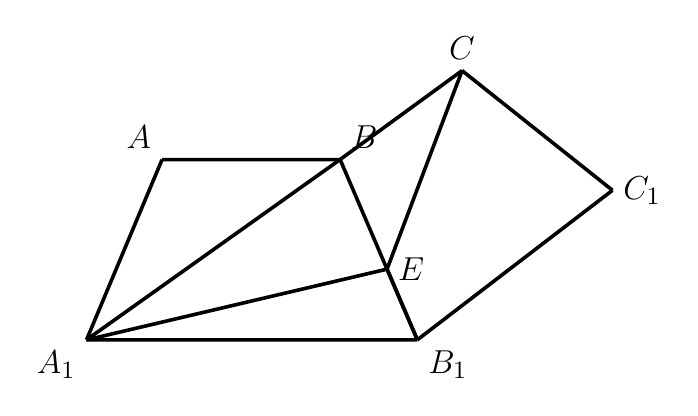
\begin{tikzpicture}[line width=1.3pt, line join=round]
  % Named coordinates (converted from pixels)
  \coordinate (A1) at (-3.3500055194240064,-1.71001135211905);
  \coordinate (A) at (-2.3899860655637455,0.5800308632414852);
  \coordinate (B) at (-0.12893160618200455,0.5804460306939089);
  \coordinate (C) at (1.420027512273642,1.7099974545247354);
  \coordinate (C1) at (3.32998582047528,0.18999869736697664);
  \coordinate (B1) at (0.8517714869122738,-1.7092398355161948);
  \coordinate (E) at (0.4671383715085607,-0.8112218581918613);

  % Segments (all solid black)
  \draw (A1) -- (A);
  \draw (A) -- (B);
  \draw (A1) -- (B) -- (C);   % A1-B-C is one straight line
  \draw (B) -- (B1);
  \draw (A1) -- (B1);
  \draw (A1) -- (E);
  \draw (C) -- (E) -- (B1);   % C through E down to B1
  \draw (C) -- (C1);
  \draw (C1) -- (B1);

  % Labels (math mode, STYLE METRICS font)
  \node[above left,  font=\fontsize{13}{15.6}\selectfont] at (A)  {$A$};
  \node[above right, font=\fontsize{13}{15.6}\selectfont] at (B)  {$B$};
  \node[above,       font=\fontsize{13}{15.6}\selectfont] at (C)  {$C$};
  \node[right,       font=\fontsize{13}{15.6}\selectfont] at (C1) {$C_1$};
  \node[right,       font=\fontsize{13}{15.6}\selectfont] at (E)  {$E$};
  \node[below left,  font=\fontsize{13}{15.6}\selectfont] at (A1) {$A_1$};
  \node[below right, font=\fontsize{13}{15.6}\selectfont] at (B1) {$B_1$};
\end{tikzpicture}
\end{document}
% GEOAGENT_REPAIR_V1 c18a466396f54661 90ac19e6b43986abd00327e43e6b3c1444c0149643691d961b1928f580dd0e01
